
À mon arrivée chez \emph{mediarithmics}, il a été décidé que mon sujet porterait sur l'optimisation de \emph{bid}. 
Ainsi, dans cette partie je vais dans un premier temps présenter qu'est ce que le \emph{Real-Time Bidding} et les 
objectifs d'un \emph{bid optimizer}. Dans un second temps, je présenterai l'analyse de la solution existante chez 
\emph{mediarithmics} pour répondre à ce problème. Dans une troisième partie je dresserai une présentation de la 
veille technologique effectuée autour de cette problématique. Ensuite, j'aborderai l'implémentation de la solution 
ainsi que son suivi en production. Enfin, j'évoquerai les pistes d'amélioration autour du travail réalisé.
\section{Online Bid Optimization} 
    \subsection{Presentation du Real-Time Bidding}
        Avant d'aborder, le sujet du \emph{bid optimizer}, il faut premièrement expliquer ce qu'est le 
        \emph{real-time bidding}. En temps réel, lorsque un internaute charge une page, avec des emplacements 
        publicitaires, ces derniers sont mis aux enchères auprès d'un \emph{Adexchange}. Un \emph{Adexchange} est 
        une plateforme automatisée d'achat et de vente en ligne et en temps réel. Elle permet donc à des 
        \emph{annonceurs}\footnote{acteurs cherchant à diffuser des publicités et achetant les emplacements} 
        et à des \emph{publishers}\footnote{acteurs affichant et vendant des emplacements} d'interragir. Prenons
        un exemple. Un \emph{publisher} possède un site internet sur lequel il a défini des emplacements 
        publicitaires. Le publisher a référencé ces emplacement auprès d'un  \emph{Adexchange}. De leurs côtés des 
        annonceurs ont indiqués à l'Adexchange leur volonté d'afficher de la publicité à des internautes. Ainsi,
        lorsque un utilisateur va venir charger une page web du site du publisher contenant un emplacement 
        publicitaire référencé, une requête est envoyée à l'Adexchange avec toutes les données disponibles sur 
        l'utilisateur ainsi que des informations contextuelles, telles que l'\emph{id} de l'emplacement ou encore 
        celui du site web. L'Adexchange va alors informer tous les annonceurs qu'un emplacement publicitaire est 
        disponible et l'enchère est ouverte. Connaissant les informations de l'utilisateur ainsi que les données 
        contextuelles, les annonceurs vont alors placer une enchère. L'annonceur ayant l'enchère la plus haute est 
        alors informé par l'Adexchange qui demande à l'annonceur gagnant quel publicité ce dernier veut afficher.
        À la vue de cet exemple, il apparaît une difficulté majeure pour les annonceurs, quelle enchère placer. Ce processus est schématisé sur la figure \ref{fig:rtb} En 
        effet en fonction de la campagne publicitaire, des informations sur l'emplacement publicitaire ainsi que 
        sur l'utilisateur, il convient de définir un prix d'achat. Il apparaît clairement la nécessité de 
        requérir à un système d'optimisation d'enchères dit \emph{bid optimizer}.
        \begin{figure}
            \label{fig:rtb}
            \centering
            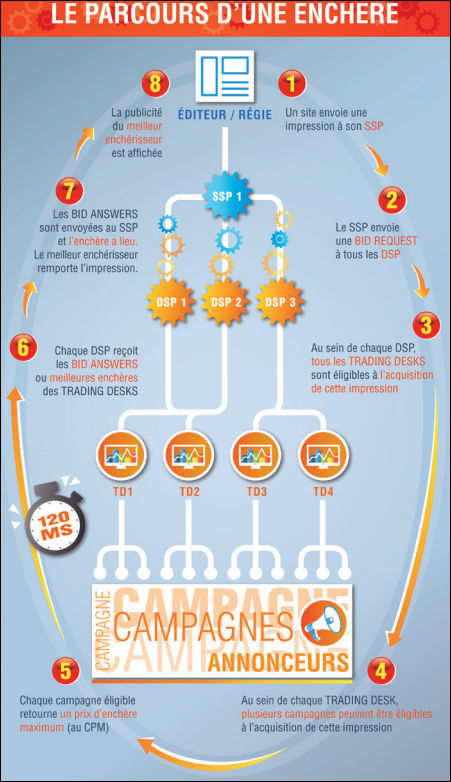
\includegraphics[scale=0.3]{images/rtb.jpg}
            \caption{Schmématisation du \textbf{RTB} \url{https://www.definitions-marketing.com/wp-content/uploads/2016/04/rtb.jpg}}
        \end{figure}
    \subsection{Objectifs d'un bid optimizer}
        Comme expliqué dans le paragraphe précédent, pour acheter une publicité sur internet, il faut répondre à une enchère. L'objectif d'un bid optimizer est donc de fixer un prix à un emplacement publicitaire donné pour un utilisateur. Mais, afin de savoir quel prix payer, il faut fixer un objectif au \emph{bid optimizer}. En \emph{data marketing}, existe le concept de \textbf{conversion}. Lorsqu'un annonceur choisit de diffuser une campagne publicitaire, il a un objectif. Cette objectif peut être varié. L'annonceur peut rechercher via sa campagne publicitaire à augmenter le nombre de personnes inscrites à sa newsletter, le nombre de vente d'un produit via son site internet, le nombre de visites sur son site. Lorsqu'une publicité est affichée, il s'agit donc de suivre l'utilisateur afin de tracker la conversion future de l'évènement. Une conversion un peu plus triviale cependant est le \emph{click}. Dans ce cas là, on va considérer que l'objectif de la campagne publicitaire est de générer le plus de clicks possibles sur la publicité affichée. On appelle cet objectif le CTR\footnote{Click-Through Rate}. Durant mon stage, c'est sur cette objectif là que mon travail sur le bid optimizer a porté. Chez \emph{mediarithmics}, un bid optimizer est considéré comme un plugin. Un plugin est un programme s'interfaçant à la plateforme \emph{mediarithmics} permettant de répondre à un besoin précis. Dans notre cas, nous pouvons considérer le RTB comme un problème à une entrée, \emph{Bid decision request} et une sortie \emph{Bid decision}, voir figure \ref{fig:bid-optimization}. Ce fonctionnement permet à la plateforme \emph{mediarithmics} d'être connecté aux divers \emph{Adexchanges} via \textbf{OpenRTB}\footnote{\url{https://openrtb.github.io/OpenRTB/}}, puis via les plugins, de permettre à ses clients de développer leurs propres \bo répondant au mieux à leur besoin. Dans le cadre de mon stage, c'est \med qui est développeur d'un plugin \bo. Pour être plus précis, nous nous sommes intéressés dans notre cas à l'optimisation de campagnes de \emph{prétargeting}\footnote{\url{https://goo.gl/qkqZKC}}. La particularité des campagnes de prétargeting est que ces dernières ne disposent pas de données personnelles sur l'utilisateur, mais seulement de données contextuelles telles que l'emplacement géographique et la date du dernier affichage publicitaire à cet utilisateur par exemple. Pour résumer, le \bo sur lequel j'ai travaillé pendant mon stage est un \bo donc l'objectif est de maximiser le click d'un utilisateur en fonction de données contextuelles. L'optimisation d'un tel objectif présente néanmoins de nombreux défis que je vais maintenant présenter.
        \begin{figure}
            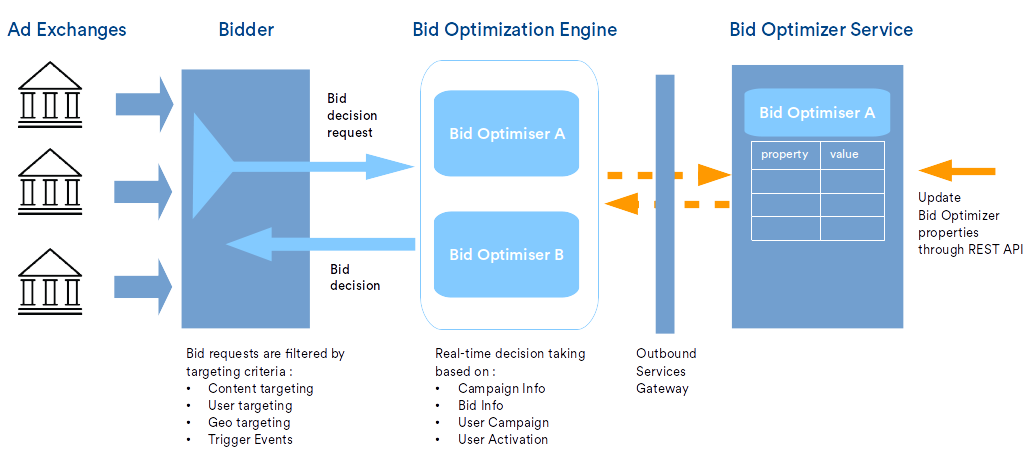
\includegraphics[width=\linewidth]{images/bid-optimization-engine-and-bid-optimizer.png}
            \caption{Schéma du concept de \textbf{bid optimizer} chez \emph{mediarithmics}}
            \label{fig:bid-optimization}
        \end{figure}
    \subsection{Défis d'un bid optimizer}
        Un \bo est un modèle prédictif prenant des paramètres en entrées et sortant un prix d'achat. L'apprentissage d'un tel modèle se fait par le biais de techniques de \emph{machine learning}. Or compte-tenu de la nature de notre cas d'utilisation, plusieurs problèmes se posent. Dans un premier temps, il faut prendre en compte la volumétrie des données. En effet, une journée de données représente plusieurs millions d'évènements. \ref{fig:bid-requests-nb}
        \begin{figure}[ht]
            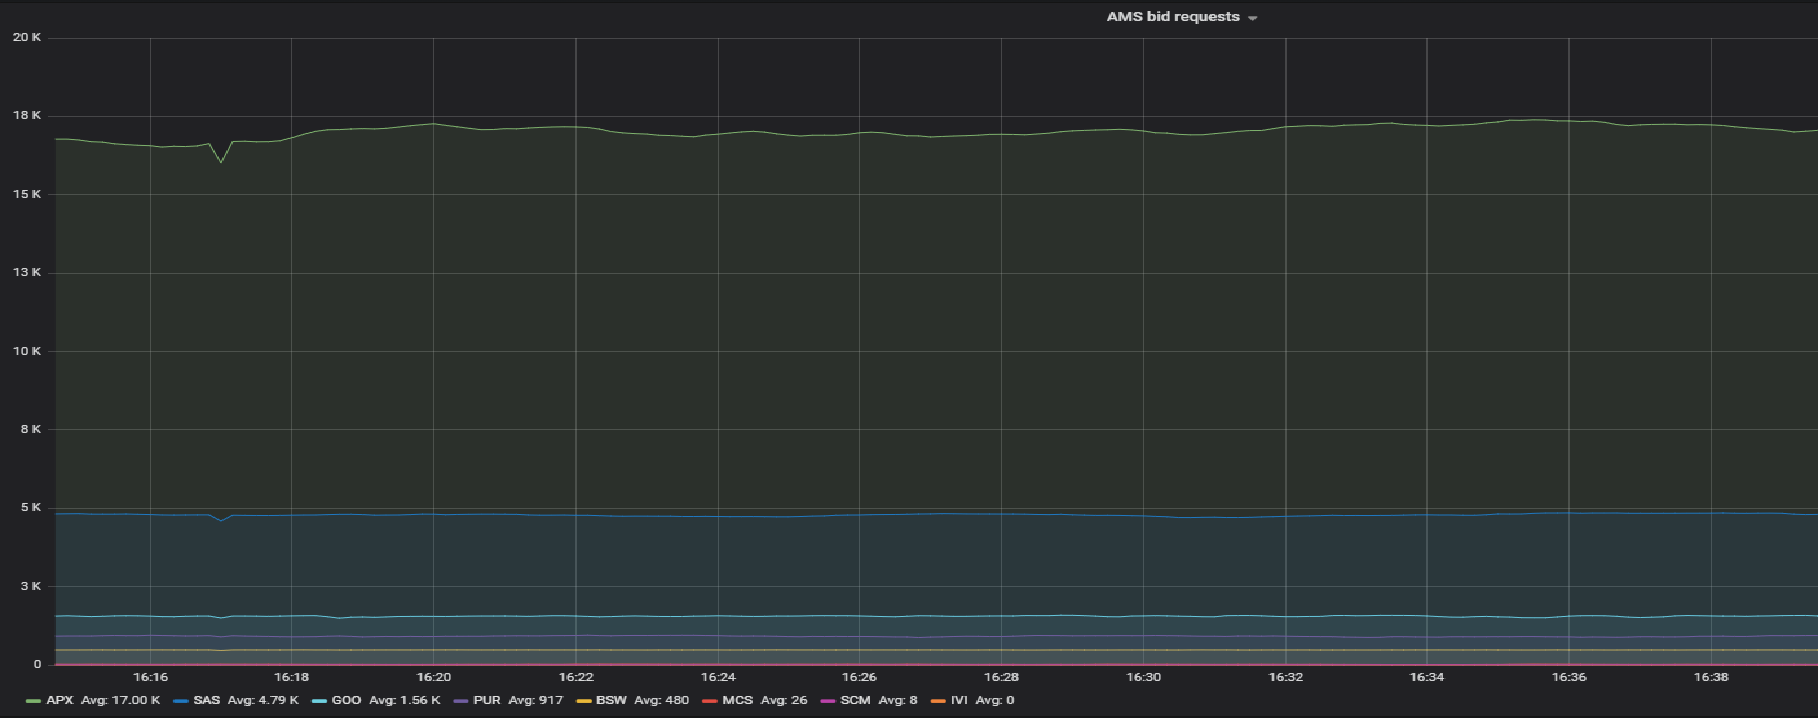
\includegraphics[width=\linewidth]{images/bidrequests.png}
            \caption{Capture d'écran de l'outil de monitoring \textbf{Grafana} représentant le nombre de \emph{bid requests} par seconde chez \emph{mediarithmics}. On observe une moyenne à 18000 requêtes par seconde en provenance de l'Adexchange d'Amsterdam}
            \label{fig:bid-requests-nb}
        \end{figure}
        Malgré cela, les cliques sont extrêmement rares, avec une probabilité de l'ordre de $10^{-4}$, ce qui crée un problème de représentation du clique dans les jeux de données d'apprentissage. De plus, le monde du \emph{data marketing} est un domaine très changeant. En effet, les publicités, tout comme les emplacements publicitaires changent par exemple. Or ce sont deux paramètres de choix à l'apprentissage d'un \bo. Plusieurs techniques existent pour contrer ce problème que nous aborderons la prochaine partie. En bref, les données relatives à l'apprentissage d'un modèle prédictif de \bo sont de haute dimension, en  très grand nombre avec une fréquence d'évènement positif extrêmement faible, et elles changent dans le temps. Ce sont tous ces facteurs qu'il faut prendre en compte lors du développement d'un \bo. Par conséquent, dans la partie suivante j'analyserai la solution développée jusqu'à lors chez \emph{mediarithmics} sur l'ensemble des points évoqués, puis je présenterai les améliorations qu'il est possible d'apporter à cette solution.
\section{Analyses de la solution existante}
    \subsection{Présentation de la solution actuelle}
    Je vais maintenant présenter la solution existante développée au sein de \med. Bien, que l'on pourrait penser au premier abord que le-dit problème est un problème de régression, il est traité comme un problème de classification. Pour un évènenement donné l'idée est d'obtenir la probabilité d'appartenance de cet évènement à la classe, puis en multipliant cette probabilité par un facteur correspondant au prix maximum que l'on est prêt à débourser pour un emplacement publicitaire. Ce prix est fixé par les clients de \med lors de la paramétrisation de leurs campagnes sur la plateforme. Le plugin développé par \med nommée \textbf{DTLR} est basée sur un papier de \emph{facebook} de 2015 \cite{he2014practical}. Historiquement le problème de prédiction de cliques est abordé via une régression logistique. En effet, les modèles linéaires ont l'avantage d'être explicatif , et rapide à entraîner ce qui correspond à la fois aux besoins métiers du \emph{data marketing} en fournissant des réponses sur l'origine de la prédiction au \emph{marketeur}, tout en répondant aux contraintes techniques contenues dans la volumétrie du problème avec un temps d'apprentissage et de prédiction faible. Néanmoins, les modèles linéaires ont des limites de modélisation. Ils ne peuvent par exemple, par définition, pas modéliser les non-linéarités. Or compte-tenu du caractère catégoriel et de la \emph{sparsité} des données, le modèle linéaire montre très vite des limites de modélisation. Par exemple, on peut imaginer que deux \emph{features} pris séparémment ne soient pas discriminants. Malgré tout  ces deux \emph{features} combinés peuvent l'être. La visite de tel ou tel site web à une heure donnée peut être corrélé au succès d'une publicité en terme de cliques alors que ce même site à une autre heure ou bien un autre site à la même heure offrent des performances moindres. On comprend ici bien le besoin de modéliser de la non-linéarité. L'idée du papier présenté par \emph{facebook} est ainsi de modéliser des \emph{features} de plus haut niveau à l'aide d'arbres de décisions et dans un second temps d'appliquer un modèle linéaire de régression logistique pour obtenir les prédictions. \med s'est donc inspiré de ce papier pour développer le \bo \textbf{DTRL}\footnote{Decision Tree Logistic Regression}. Le principe est identique à celui évoqué dans le papier. 
Ainsi le \bo initialement développé a les spécificités suivantes. Dans un premier temps, il est paramétrable via un fichier de configuration. Ce fichier de configuration permet à la fois de choisir les variables d'entrée du modèle ainsi que les preprocessings associés, comme par exemple une transformatiom logarithmique ou bien l'explosion d'un feature \emph{timestamp} en plusieurs features comme le jour de la semaine et une tranche horaire.
Également, ce fichier de configuration permet de chosir entre deux modes d'apprentissage. Un premier mode qui consiste en l'apprentissage d'un modèle de régression logistique standard (\textbf{LR}) et un deuxième mode qui consiste en l'apprentissage d'un modèle d'arbre de décisions suivis d'une régression logistique (\textbf{DTLR})comme présenté précedemment. 
À partir de ces fichiers de configurations, les clients ont la possibilité de personnaliser leurs apprentissages. Par la suite, chaque nuit, un nouveau modèle est appris sur les données des $N$ derniers jours. Ce modèle est ensuite publié en production pour servir de \bo pour la journée à venir. 
Côté implémentation, cette dernière a été effectuée par une combinaison de \emph{Scala}\footnote{\url{https://www.scala-lang.org/}}, et scripts \emph{bash}\footnote{\url{https://fr.wikipedia.org/wiki/Bourne-Again_shell}}.
L'apprentissage d'un modèle consiste en une succession d'exécutions de scripts \emph{Scala} de l'appel à des exécutables de librairies externes. Le script shell d'apprentissage est premièrement lancé avec un paramètre nombre de jours $N$. Dès lors, une succession de scripts \emph{scala} s'occupe de récupérer les données des $N$ derniers jours, puis de les pré-traiter. À partir de là, à partir du fichier de configuration, soit est lancé un apprentisage de \textbf{LR}, soit un apprentissage de \textbf{DTLR}. Les librairies utilisées pour réaliser les apprentissages des arbres de décision et de la régression logistique sont \textbf{Xgboost}\footnote{\url{lhttps://github.com/dmlc/xgboost}} \cite{Chen:2016:XST:2939672.2939785} et \textbf{Vowpal Wabbit}\footnote{\url{https://github.com/JohnLangford/vowpal_wabbit/}} \cite{langford2009sparse} réciproquement. Afin de mesurer la qualité de l'apprentissage la métrique \emph{AUC-ROC}\footnote{Area Under the Curve - Receiver Operating Characteristic} est utilisée. Une courbe \textbf{ROC} est une courbe représentant le taux de vrais positifs avec le taux de faux positifs. Pour différents seuils de classification, on peut alors calculer les taux de vrais positifs et les taux de faux positifs pour un ensemble de prédictions données. Par conséquent, on peut calcule une mesure aggrégée des performances pour tous les seuils de classifications, ce qui correspond à l'aire sous la courbe \textbf{ROC}. L'\textbf{AUC} est une métrique particulièrement appréciée pour tous les problèmes de classification avec une répartition des classes déséquilibrée. Une comparaison de différentes métriques a été effectuée sur des problèmes d'optimisation d'enchères et il en ressort la pertinence du choix de cette métrique dans notre cas d'utilisation \cite{yi2013predictive}. Maintenant que j'ai expliqué en détail la conception de la solution du \bo, je vais maintenant aborder les limites principales de cette dernière. 
    \subsection{Axes d'amélioration}
        Bien que répondant aux critères initiaux d'un \bo, \textbf{DTLR-LR} a cependant quelques défauts. Le premier est celui de la maintenabilité. En effet, comme explicité plus haut, l'apprentissage et le déploiement du modèle est dépendant de deux librairies tierces. De surcroît, cette utilisation de librairies tierces se fait via des appels systèmes appartenant à un \emph{pipeline} de traitement décrit dans un script shell. La communication entre scripts \textbf{Scala} et appels systèmes se fait par le biais de fichiers texte. Cet enchevêtrement d'opérations rend par conséquent compliqué le test du \textbf{plugin}, ou bien encore la montée en version des librairies tierces, par exemple, si dans un changement de version, le format des entrées ou bien des sorties est modifié. De plus, cela rend également très difficile l'ajout potentiel de traitements supplémentaires permettant d'améliorer l'algorithme. \par De plus un autre problème de cette solution est le temps d'apprentissage des modèles. Une optimisation étant basée sur les $N$ derniers jours de données, et une journée de donnée pouvant contenir plusieurs millions d'évènements, cela résulte en des apprentissage de plusieurs heures. \par
        Enfin comme évoqué notamment dans le papier de \emph{facebook} \cite{yi2013predictive}, les performances des modèles d'optimisation d'enchères sont fortement corrélées à la fraîcheur des données d'apprentissage. \par 
        % Problème du temps d'apprentissage
            % Temps d'apprentissage de DTLR très long si nmbre de jours pris en compte élevé compte tenue de la volumétrie
        % Abord du problème de data freshness nottamment évoqué dans le papier de facebook.
        % Ouverture sur la partie suivante
    \subsection{Définition des problématiques et contours du problème}
        Des axes d'amélioration évoqués dans la partie précédente se dégagent trois problématiques autour de l'amélioration du \bo que j'ai eu l'opportunité d'aborder pendant la durée de mon stage. \par 
        Le premier est la mise en place d'un mode \emph{online} du \bo existant. Cela consiste au développement et à l'intégration à \textbf{DTLR-LR} d'une manière d'apprendre le modèle en ligne. L'objectif de cette amélioration est ainsi d'offrir aux utilisateurs du plugin \textbf{DTLR-LR}, la possibilité d'entraîner un modèle en ligne de régression logistique. Il aurait pu également être envisagé de proposer un mode d'apprentissage en ligne pour \textbf{DTRL}, en approfondissement l'implémentation initiale comme suggéré dans \cite{yi2013predictive} en effectuant l'apprentissage des arbres de décisions sur un intervalle de temps plus long tout en apprenant la régression logistique en ligne. \par
        Le deuxième axe d'amélioration consiste en la recherche et le développement de nouveaux modèles de \bo. L'objectif ici, est de faire des tests sur les algorithmes de machine learning à l'état de l'art et d'étudier la faisabilité de leur implémentation et intégration au sein de l'architecture \med. \par 
        Le troisième objectif d'amélioration sur lequel j'ai travaillé est sur la modularité et maintenabilité de \textbf{DTLR-LR}. Cet amélioration consiste à l'étude et à un \emph{POC} sur la faisabilité d'implémenter l'apprentissage d'un \bo en s'affranchissant du \emph{pipeline} de traitement décrit actuellement dans le script \emph{shell} mentionné auparavant. en des termes d'informatique logicielle, il est donc question de \emph{refactorer} le code existant, sans introduire de régression par rapport au fonctionnement préalable du \bo et en gardant des performances comparables. \newline \newline
    
    Comme je viens juste de le décrire mon stage a porté sur l'amélioration du \bo autour des trois critères définis dans le précédent paragraphe. La démarche que je vais suivre afin de présenter mon travail pour chacune de ces améliorations est la suivante. Pour chaque amélioration, je présenterai dans un premier temps la veille technologique et la recherche que j'ai effectué en amont. Puis je présenterai les différentes implémentations et \emph{POC} que j'ai effectué pour répondre aux besoin définis. Enfin je dresserai un bilan critique de chacun de ces résultats, et évoquerai des pistes d'évolution possibles.
        
        % Objectifs d'amélioration du bid optimizer
            % Premier objectif court-termiste: développement d'un mode online avec performances équivalentes
            % Deuxième objectif: réflexions et présentation de la recherche autour de l'amélioration des performances par l'exploration et le test de d'autres modèles / librairies de machine learning (catboost - tensorflow...). Présenter les tests effectués via catboost et tensorflow en expliquant les raisons du rejet de la solution: lisibilité métier, performances pas assez intéressantes pour justifier un tel effort d'implémentation. Problème de déploiement du modèle au sein de l'architecture (human readables modèles en sortie par exemple)
            % Troisième objectif: réflexions et tests autour de l'amélioration de la modularité et et de la maintenabilité du plugin. Expliquer la tentative d'implémentation de la descente de gradient / logistique régressions avec les librairies de l'écosystème Scala telles aue Nak, breeze etc.. et insister sur l'immaturité du langage pour effectuer du machine learning.
\section{Ajout d'un mode online à DTLR-LR}
    % Besoin de comprendre le comportement du bid optimizer en production -> recherche sur VW et les optimizers associés pour comprendre le fonctionnement
    La solution actuelle, \textbf{LR} utilise \emph{Vowpal Wabbit} comme évoqué précedemment. \emph{Vowpal Wabbit} est une librairie de machine learning spécialisée dans l'apprentissage de modèles en ligne. Initialiement développé par John \textsc{Langford} au sein des laboratoires de recherche de \emph{Yahoo!}, la librairie est dorénavant maintenue par \emph{Microsoft}. Sa force réside dans sa capacité à traiter des données \emph{sparses} de haute dimensionnalité. C'est dans cette optique qu'à dans un premier temps été choisie cette librairie lors de l'implémentation initiale de \textbf{DTLR-LR}. Néanmoins, les possibilités d'apprentissage de modèles en ligne n'étaient pas encore exploitées. C'est ce point que je vais donc évoquer dans cette partie. 
    \subsection{Veille technologique}
        Dans un premier temps je vais présenter les \emph{features} essentiels qui font de \emph{Vowpal Wabbit} une solution de choix pour notre cas d'utilisation. \par
        La première fonctionnalité qui fait de \emph{Vowpal Wabbit} un bon choix et la \text{Truncated Gradient Descent} \cite{langford2009sparse}. Lorsque l'on apprend un modèle linéaire, cela veut dire que l'on apprend un au moins un poids par \emph{feature}, comme c'est le cas lors d'une régression logistique. Dans des espaces en haute dimension par exemple avec un jeu de données avec $10^6$ \emph{features}, le modèle a $10^6$ paramètres. Or dans ces jeux de données de haute dimensionnalité, la plupart des \emph{features} sont rares et ne sont pas discriminants tandis qu'une très petite minorité de \emph{features} a de l'importance. Malgré tout, ce sont l'ensemble des caractéristiques du modèle qui rentrent en compte lors de l'apprentissage avec la descente de gradient et lors de la prédiction. Cela crée deux problèmes majeurs. Le premier est la taille du modèle. Effectuer un apprentissage sur un modèle avec $10^6$ caractéristiques suppose de charger en mémoire à la fois l'ensemble des caractéristiques du modèles mais à la fois l'ensemble des caractéristiques des exemples d'apprentissage. Cela est bien souvent impossible ou bien limite à un apprentissage par \emph{batch} de taille réduite. Le deuxième problème est celui du temps d'apprentissage et d'inférence. En effet, plus il y a de paramètres, plus les calculs sont longs. Il y a donc une volonté pour ces modèles, d'induire de la \emph{sparsité} dans le modèle. Concrètement, ce que cela signifie est que l'on va chercher à fixer à zéro les paramètres du modèle ayant une faible importance dans la décision (la majorité). Par conséquent, l'on peut par la suite effectuer des calculs d'apprentissage et d'inférence efficace. C'est l'objectif fixé par le papier de John \textsc{Langford}. Le papier s'inspire donc de deux idées principales. La première est celle de l'algorithme du \textbf{Lasso}. Le lasso permet de faire tendre des poids du modèles à zéro. La deuxième idée, décrite dans le papier comme trop \fg aggressive \og. La \emph{Truncated Gradient Descent} propose donc de mixer ces deux idées par l'introduction d'un hyper-paramètre nommé \emph{gravité}. Cet hyper-paramètre va permettre de diminuer à l'image du lasso, la norme des poids des features. Puis l'algorithme de descente de gradient va arrondir à zéro les features descendant en dessous d'un certain seuil. L'expérience présentée dans le papier consiste en l'utilisation de jeu de données de la base de données  \text{UCI}\footnote{https://archive.ics.uci.edu/ml/datasets.html} auxquels ont été ajoutés des caractéristiques aléatoires, qui n'ont par conséquent pas de corrélation avec les labels. Puis, en comparant une descente de gradient standard avec une \emph{Truncated Gradient Descent}, ils parviennent à obtenir des modèles entre $70\%$ et $90\%$ réduits tout en gardant des performances équivalentes. Cette descente de gradient particulière est donc implémentée nativement dans \emph{Vowpal Wabbit}. \par
        La deuxième fonctionnalité est l'implémentation native de l'optimizer \textbf{ADAGRAD}\footnote{ADaptive GRADient descent}\cite{duchi2011adaptive}. Ce papier introduit un nouvelle algorithme de descente de gradient. De nouveau, les bénéfices de cet algorithme résident dans son adaptation aux jeux de données en haute dimension. L'idée est de donner aux caractéristiques les moins fréquentes des taux d'apprentissages élevés et réciproquement aux caractéristiques les plus fréquentes des taux d'apprentissages plus bas. Dans l'algorithme standard de la descente de gradient tous les paramètres sont mis à jour en multipliant le gradient par un taux d'apprentissage fixe et partagé. Avec \textbf{ADAGRAD}, un taux d'apprentissage différent pour chaque paramètre du modèle existe. En effet, pour chaque itération $t$ de la descente de gradient, il est stocké la somme des carrés de tous les gradients précédents notée $G_{t, i} = \sum_{k = 0}^{t} g_{k, i}$ pour chaque paramètre $i$. Ainsi, on peut supposer que plus  $G_{t, i}$ donné est élevé pour un paramètre, plus ce paramètre a été mis à jour auparavant lors de la descente de gradient. Inversement, si un paramètre n'a jamais été rencontré,  $G_{t, i} = 0$. Dès lors, en divisant le taux d'apprentissage initial d'un paramètre $i$ par $\sqrt{G_{t, i}}$, on a un taux d'apprentissage du paramètre $i$ qui diminue au fur à mesure de l'apprentissage plus ce dernier est mis à jour. Ce fonctionnement est particulièrement adapté avec des données \emph{sparses} puisque l'on souhaite donner leur \fg chance \og aux nouveaux paramètres. De plus, de part la volonté d'effectuer un apprentissage en ligne, il est important de s'assurer de la stabilité de notre modèle. Ainsi, il est rassurant que notre optimiseur mette à jour moins fortement les paramètres les plus importants et fréquents de notre modèle. Par exemple, imaginons qu'une anomalie en production vienne à fortement changer la répartition de nos données sur un paramètre particulièrement important de notre modèle, on ne souhaite pas mettre à jour fortement notre modèle dans la direction de l'anomalie. D'autre part, l'intégration d'un nouveau paramètre au modèle comme de nouveaux sites ou bien de nouvelles publicités sera correctement assimilée par le modèle car ces derniers auront la possibilité d'exprimer leur potentiel discriminant face aux \fg vieux \og paramètres. \par
        Je viens ici d'exprimer les principaux bénéfices de l'implémentation de \emph{Vowpal Wabbit}. Dans un contexte professionnel et dans un environnement de production le contrôle de la stabilité du modèle ainsi que sa compréhension. Je vais maintenant présenter mon travail d'implémentation en production d'un apprentissage de régression logistique en ligne.
    \subsection{Implémentation de la solution}
        Avant de faire l'effort de développer une nouvelle fonctionnalité dans un environnement de production au sein d'une entreprise, il faut dans un premier temps s'assurer que cette dernière est faisable, et se comporte comme souhaité initialement lors de la phase de spécifications. C'est ce que j'ai dans un premier temps effectué. Avant de développer la version opérationnelle du bid optimizer en ligne. Il a fallu s'assurer de deux choses principales. Premièrement, les performances sont comparables avec celles de \textbf{DTLR-LR} en mode batch. Deuxièmement, être sûr de maîtriser le modèle et l'apprentissage afin d'être en mesure de comprendre le modèle dans l'environnement de production. \par
        Pour commencer, j'ai donc voulu dans un premier temps m'assurer de la possibilité de faire de l'apprentissage en ligne avec \emph{Vowpal Wabbit}. J'ai donc élaboré un processus de traitement afin d'effectuer cette première simulation que voici:
        \begin{itemize}
            \item Choisir un jeu de données. En effet, peut importe le jeu de données dans cette étape, il s'agit avant tout de démontrer la capacité de \emph{Vowpal Wabbit} d'apprendre en ligne. Pour cela la librairie doit être capable de faire deux choses:  sauvegarder le modèle et son état et reprendre l'apprentissage à partir d'un état précédent
            \item Diviser le jeu de données en deux: un jeu de données de test et un jeu de données d'apprentissage. 
            \item Diviser le jeu de données d'apprentissage en \emph{batchs} de taille équivalente. Cela va nous permettre à la fin de chaque \emph{batch} de mesurer la performance du modèle. En effet, un apprentissage en ligne peut être assimilé à un apprentissage par \emph{}batch, si l'on enregistre le modèle à la fin de chaque \emph{batch} et l'état de l'apprentissage. De cette façon, il est possible de repartir des poids du modèle du \emph{batch} précédent.
            \item Pour chaque \emph{batch}, charger le modèle du \emph{batch} précédent, puis effectuer l'apprentissage sur les données du \emph{batch}.
            \item Calculer le coût moyen d'apprentissage sur le \emph{batch}, puis le coût en validation. 
            \item Tester le nouveau modèle sur les données de test afin de calculer la métrique de test.
        \end{itemize}
        Avec cette procédure, il y a deux choses que sur lesquelles on veut s'assurer. Premièrement le fait, que la courbe d'apprentissage est normale, c'est à dire que le coût diminue de manière constante. Cela permet de s'assurer des capacités de \emph{Vowpal Wabbit} de sauvegarder un modèle et de redémarrer l'apprentissage. Deuxièmement, on veut s'assurer que les variations de coût sont cohérentes avec les variations de la métrique de test. Plus clairement, une baisse du coût en validation, entraîne une amélioration de la métrique de test. \par
        J'ai donc choisi un jeu de données \emph{Higgs} sur le site \textbf{UCI}\footnote{\url{https://archive.ics.uci.edu/ml/datasets/HIGGS}}, auquel j'ai appliqué le processus de traitement explicité juste dessus. Pour ce faire, j'ai implémenté une série de scripts \emph{python} permettant et de scripts \textbf{shell} permettant de diviser les jeux de données de manière équitable, c'est à dire en conservant les répartitions des classes, de pré-traiter les données au format \emph{Vowpal Wabbit}\footnote{\url{https://github.com/JohnLangford/vowpal_wabbit/wiki/Input-format}} qui est un format proche du format \textbf{libsvm}, format permettant de représenter les jeux de données avec une représentation sparse. Les résultats de cette première expérience sont présentés en figure \ref{fig:exp_outliers_first}. 
        \begin{figure}[h]
            \label{fig:exp_outliers_first}
            \centering
            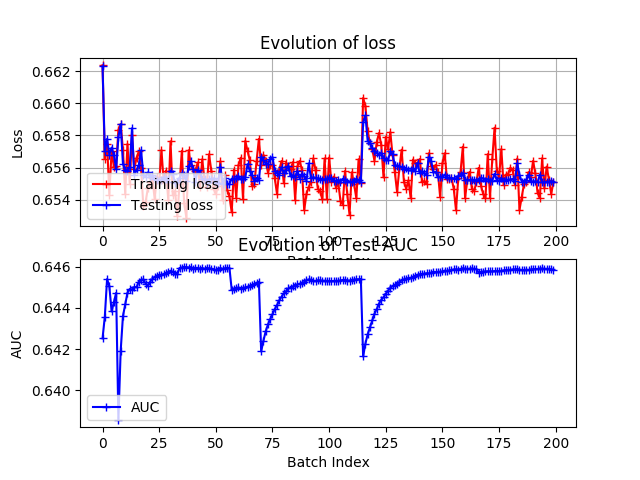
\includegraphics[scale=0.75]{images/experiment_outliers_first.png}
            \caption{Représentation d'un apprentissage en ligne avec vowpal wabbit avant nettoyage des outliers}
        \end{figure}
        On peut voir sur cette figure que l'on obtient une courbe d'apprentissage standard résultant d'une descente de gradient. Plusieurs points éveillent toutefois l'attention. Le premier est le bruit du coût d'apprentissage. Ce dernier s'explique simplement. A la différence du jeu de données de test qui est fixe, le jeu de données d'apprentissage change à chaque \emph{batch}. Or le coût d'apprentissage représenté sur le graphe correspond au coût moyen du \emph{batch}. Il est donc cohérent d'obtenir un signal bruité. Le deuxième point qui mérite notre attention sont les deux chutes de performances lors du \emph{batch} $70$ et $110$. Il convient de comprendre l'origine de ces deux évènements, afin de s'assurer de la stabilité de l'apprentissage. J'ai par conséquent développé des scripts permettant d'obtenir des statistiques descriptives sur les données. J'ai ainsi pu, pour chacun des \emph{features}, représenter un diagramme à moustache à partir d'un échantillon aléatoire du jeu de données d'apprentissage. Il est visible en figure \ref{fig:box-plot-train} un exemple du résultat pour une caractéristique. 
        \begin{figure}[h]
            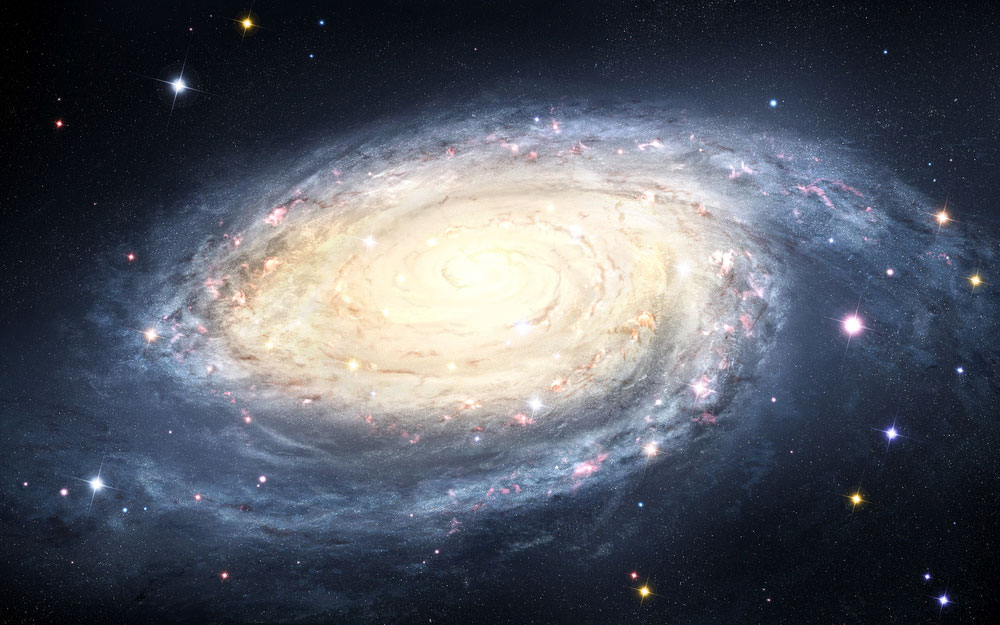
\includegraphics[width=\linewidth]{images/universe.jpg}
            \caption{Boîte à moustache du feature FEATURE A INDIQUER sur un échantillon aléatoire de l'ensemble du jeu de données d'apprentissage}
            \label{fig:box-plot-train}
        \end{figure}
        Puis, les mêmes statistiques descriptives peuvent être effectuées sur les batchs seuls. En l'occurence, je me suis intéressé ici aux batchs $70$ et $115$. L'idée est d'essayer de déceler des \emph{outliers}. Un \emph{outlier} est un échantillon d'un jeu de donnée qui s'éloigne de la distribution des autres observations. Ainsi comme on peut le voir sur la figure \ref{fig:box-plot-train-115}, on observe des points s'éloignant de la distribution observée en figure \ref{fig:box-plot-train}.
         \begin{figure}[h]
            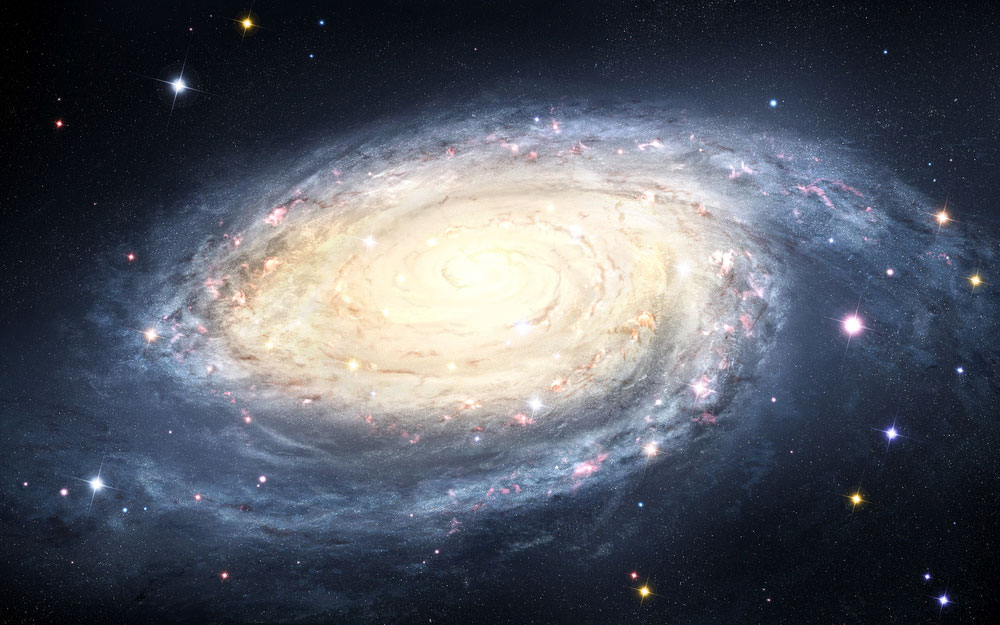
\includegraphics[width=\linewidth]{images/universe.jpg}
            \caption{Boîte à moustache du feature FEATURE A INDIQUER sur le batch 115}
            \label{fig:box-plot-train-115}
        \end{figure}
        Il semble donc que ou ou plusieurs \emph{outliers} aient pu causer cette chute de performance du modèle lors de l'apprentissage en ligne. Afin de confirmer, cette hypothèse, il faudrait relancer un apprentissage identique, en enlevant ces fameux \emph{outliers} et observer la courbe d'apprentissage résultante de cette opération. Pour trouver ces derniers, il faut trouver les points dont la distance est la plus élevée avec la valeur moyenne. En haute dimension, une distance recommandée est la distance de \textbf{Mahalanobis}\footnote{\url{https://en.wikipedia.org/wiki/Mahalanobis_distance}}. La démarche est ensuite la suivante. On prélève un échantillon aléatoire d'exemples issus de l'ensemble des données d'apprentissage, puis, pour les \emph{batch} (en l'occurence les \emph{batchs} $70$ $115$) dans lesquels on veut s'assurer que les \emph{outliers}  ne pénalisent pas le modèle , on va calculer une distance de Mahalanobis par rapport au vecteur moyen exprimé calculé. Puis, j'ai défini un seuil, ici 10\%, au delà duquel je considère le point comme un \emph{outlier} si la distance par rapport au vecteur moyen dépasse ce seuil. Il reste maintenant à relancer l'apprentissage. Comme on peut le voir sur la figure \ref{fig:exp_outliers_last}, le tri des \emph{outliers} confirme que ces derniers sont sources de perturbation dans l'apprentissage. 
        \begin{figure}[h]
            \label{fig:exp_outliers_last}
            \centering
            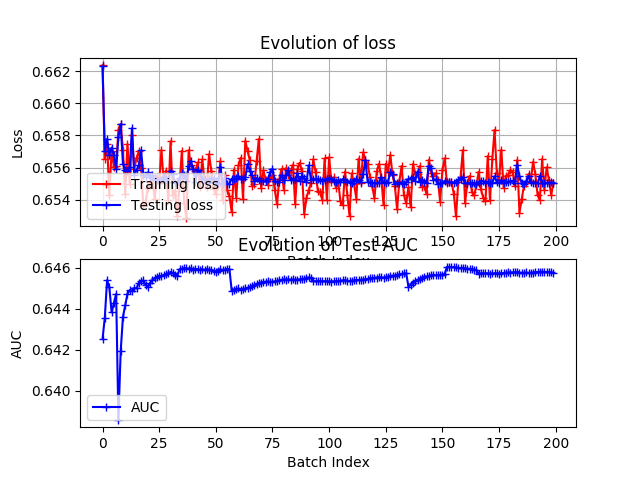
\includegraphics[scale=0.75]{images/experiment_outliers_last.png}
            \caption{Représentation d'un apprentissage en ligne avec vowpal wabbit après nettoyage des outliers}
        \end{figure}
        \par
        % Rajouter partie de comparaison entre modèles LR-HS/DTLR et 
        Maintenant, que nous avons analysé et testé les performances de \emph{Vowpal Wabbit} sur un jeu de données \fg fictif\og, testons la même procédure sur un vrai jeu de données d'une campagne publicitaire chez \med. J'ai donc agrégé des journées de campagne publicitaire de notre client \emph{BlaBlaCar}. En appliquant le même processus, on obtient le résultat visible en figure \ref{fig:exp_blabla}. 
        \begin{figure}[h]
            \label{fig:exp_blabla}
            \centering
            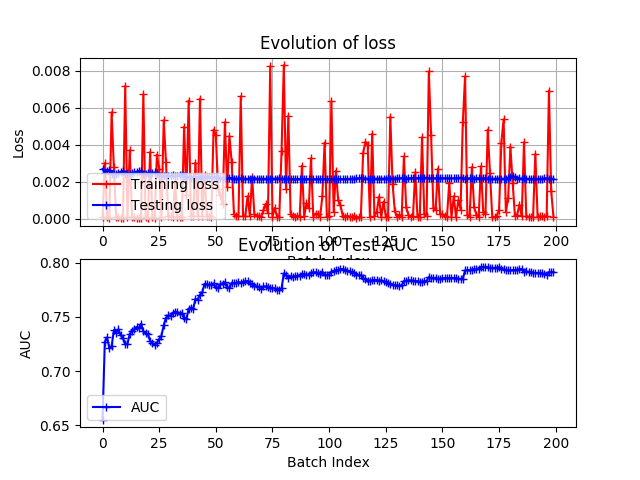
\includegraphics[scale=0.75]{images/blabla_exp.png}
            \caption{Représentation d'un apprentissage en ligne avec les données d'une campagne de BlaBlaCar}
        \end{figure}
        On observe, comme lors de l'expérience précédente que la métrique de test à savoir dans notre cas l'\textbf{AUC}. Cependant, à la différence de avec le jeu de données \textbf{HIGGS}, il semble au premier abord que le coût ne suit pas une trajectoire standard. Il ne faut cependant pas oublier la nature de notre problème, où les exemples positifs ont une probabilité d'occurrence de l'ordre de $10^-4$. Dans ces cas extrême, le coût d'apprentissage est très souvent très bas dès le départ. \par
        Après s'être assuré de la fiabilité de \emph{Vowpal Wabbit} pour notre cas d'utilisation il a donc fallu l'intégrer à la version existante de \textbf{DTLR-LR}. La première étape de l'intégration à la version existante du \bo \textbf{DTLR-LR} a été la modification du fichier de configuration permettant de paraméter l'apprentissage. En effet, en plus d'offrir la possibilité de choisir entre un modèle \textbf{DTLR} et un modèle \textbf{LR}, le fichier de configuration devait offrir la possibilité d'effectuer l'apprentissage \emph{en batch} ou \emph{en ligne}. De plus, il a fallu adapter le code existant pour s'assurer de la sauvegarde du modèle dans un format qui permette la reprise de l'apprentissage tout en permettant l'inférence. Cela est passé par la mise à jour du \emph{pipeline} d'apprentissage ainsi que de la modification du code \emph{Scala} \par
        Suite à l'implémentation de la solution est intervenue l'étape de suivi en production. Quelques semaines après la mise en production, nous avons eu l'opportunité de tester cette nouvelle version du \bo par l'intermédiaire d'une campagne de \emph{pré-targeting} d'un de nos clients/ \emph{Primagaz}. Comme il est visible sur la figure \ref{fig:primagaz}, on peut associer une vraie amélioration du taux de clicks sur la campagne suite au branchement du \bo sur la campagne.
        \begin{figure}[h]
            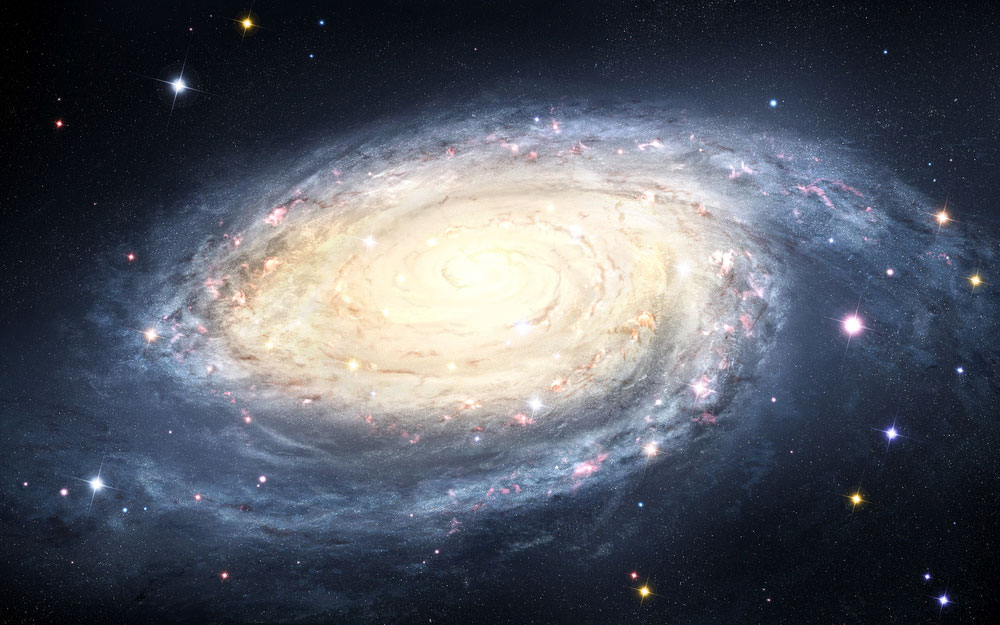
\includegraphics[width=\linewidth]{images/universe.jpg}
            \caption{Comparaison des résultats d'une campagne publicitaire avant et après branchement du bid optimizer ONLINE}
            \label{fig:primagaz}
        \end{figure}
        %Je ne rentrerai pas dans les détails de l'implémentation mais je veux néanmoins revenir sur deux difficultés que j'ai rencontré lors de cette implémentation. La première difficulté est celle de la gestion du \emph{feature hashing}\footnote{\url{https://en.wikipedia.org/wiki/Feature_hashing}}. En effet, lorsque l'on apprend un modèle avec nos données, on ne connaît pas par avance tous les \emph{features}. Par exemple
        Dans la dernière partie de cette section, je vais revenir sur les objectifs initiaux du \bo online en terme d'amélioration et conclure si les critères sont bien respectés. De plus, j'aborderai les aspects qui n'ont pas été abordés ou pris en compte par mon implémentation.
       
        % Implémentation dans l'architecture existante.
        % Modification du fichier de configuration existant pour rajouter un mode d'apprentissage.
        % Stockage des modèles lisibles en base de donnée.
        % Problème avec le hashing des features. Car le modèle d'inférence est créé programatiquement en scala cf plugin-dtlr -> nécessiter de stocker les features ainsi que leurs hash.
        % Comparaison des résultats avec DLTR et LR HS 
    \subsection{Critique et pistes d'évolution}
        
        % Réflexion sur la régularisation 
            % Objectif, optimisation en ligne, performances comparables avec apprentissage rapide ok.
            % On y a réfléchi mais pas de solutions satisfaisantes encore trouvée / implémentée
                % Apprendre un ensemble de modèles différents en même temps et sélectionner le meilleur modèle à l'instant t ce qui est rendu possible grâce à la vitesse d'apprentissage. 
        % Autres algorithmes d'optimisation et améliorations du feature engineering -> partie suivante.
            % Validation en ligne ? 
    
\section{Recherche de nouveaux modèles d'optimisation d'enchères}
    % Nouvelles approches algos pour faire de l'optimisation de bid % Objectifs 5 pages.
    \subsection{Veille technologique}
    % Kaggle -> FFM
    % Revue de l'article de google
    % Catboost -> Choix à tester
    % Feature engineering avec les outils développés par tensorflow
    \subsection{Implémentation de la solution}
        % Performance intéressante mais immaturité de la solution. En terme d'export et de lisibilité du modèle
        % Impossible à utiliser en l'état, mais piste intéressante de solution.
    \subsection{Critique et pistes d'évolution}
        
    
\section{Amélioration de la modularité et maintenabilité de DTLR/LR}
    % All the shit about nak / breeze / stuff pour implémenter une descente de gradient soit même avec scala
    \subsection{Veille technologique}
    \subsection{Implémentation de la solution}
    \subsection{Critique et pistes d'évolution}

\subsection{Trouver un nom à cette partie}
    % Ce qu'il reste à faire, conclusion plus générale sur les difficultés de ce projet, plus idées d'amélioration et travail en cours comme la réflexion autour d'une métriqué d'évaluation des bids optimizers chez mediarithmics plus pertinente ou encore la conception d'un jeu de test standardisé répondant aux besoins d'un modèle online mais également sur les réfléxions autour des nouveaux bids optimizers chez mediarithmics avec données de campagnes mutualisées par exemple.
